\subsection{Where headroom exists: synthetic populations with known truth (C3)}
\label{sec:synth}
The real pools leave almost no headroom for the mean, so we ask where shortening is possible at all in populations whose truth and best control variate are known.
$X\sim N(0,I_5)$, $\mu(X)=X_1+\tfrac12X_2$ and $f=\mu(X)$ unless stated. The \emph{knob family} sets $E[Y|f]=\cos\phi\,z+\sin\phi\,(z^2-1)/\sqrt2$ with $z$ the standardised $f$:
$\phi=0^\circ$ is a calibrated predictor (no headroom) and $\phi=90^\circ$ a purely quadratic dependence that no affine map of $f$ can use.
The named scenarios are \texttt{calibrated}; \texttt{heavy\_tail} (calibrated, $t_3$ noise); \texttt{monotone\_miscal} ($E[Y|f]=\mathrm{logit}\,f$ up to scale); \texttt{nonmonotone} ($E[Y|f]=f^2-\mathrm{const}$);
\texttt{X\_informative} ($Y$ depends on a feature $f$ misses); \texttt{subgroup\_bias} ($f$ biased by $+1.5$ on a subgroup);
\texttt{f\_noise\_X\_informative} ($f$ is pure noise, $X$ carries the signal); and \texttt{pure\_noise} (neither carries signal).
We use $n\in\{50,100,200,500,1000\}$ (knobs) or $\{50,200,500\}$ (named), $\rho\in\{1,0.1\}$, and 2000 (knobs) or 1000 (named) repetitions. The \texttt{oracle} control variate uses the true $E[Y|f,X]$; it is not implementable, and is the bound for adjusters of the classes of Sec.~\ref{sec:method}.
Ratios are paired width ratios against Wald PPI++ (Wald against Wald).

\begin{figure}[t]
\centering
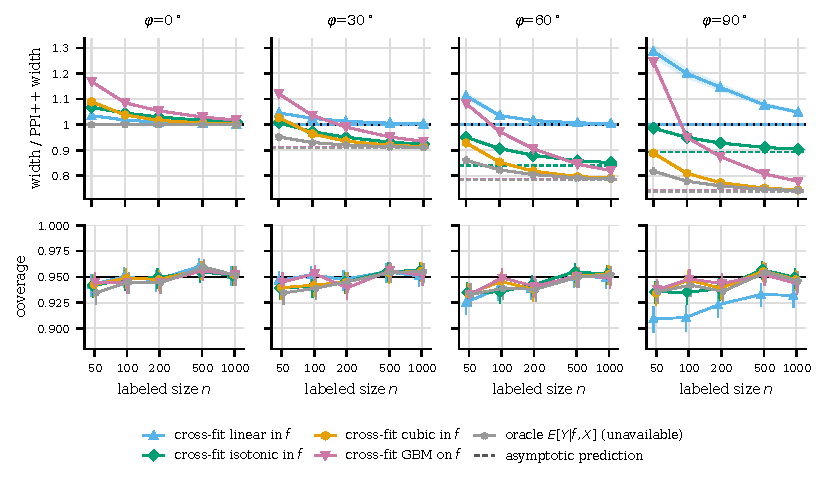
\includegraphics[width=\linewidth]{figures/fig_c3_synth.pdf}
\caption{Knob family at $\rho=0.1$ ($N=10n$), 2000 repetitions per cell, known truth. Top: paired width ratio to Wald PPI++ (solid, 95\% band); dashed horizontal lines: asymptotic prediction for the best adjuster of the class; grey: oracle $E[Y|f,X]$. Bottom: coverage with Wilson bars. The headroom appears only above a threshold $n$ that grows with the flexibility of the adjuster. Other scenarios and $\rho=1$: Appendix~\ref{app:figs}.}
\label{fig:c3}
\end{figure}

\emph{Theory.} The asymptotic ratio of Sec.~\ref{sec:theory} predicts the oracle's measured ratio closely once $n\ge200$: in the 56 cells with $n\ge200$ the measured oracle ratio exceeds the prediction by a median of 0.05\% and at most 6.6\%
(\texttt{nonmonotone}, $\rho=0.1$, $n=200$), and in the 32 cells with $n\le100$ by at most 22.5\% (\texttt{nonmonotone}, $n=50$). For the knobs $\phi=30^\circ,60^\circ,90^\circ$ at $\rho=0.1$, $n=1000$ the oracle is 0.912, 0.788 and 0.743 times as wide as PPI++, against predicted 0.910, 0.784 and 0.738;
at $\rho=1$ it is 0.961, 0.894 and 0.866 against 0.961, 0.894 and 0.866. The attainable saving is thus a property of the population and of $\rho$: up to 26\% at $\rho=0.1$ and 13\% at $\rho=1$ across the knobs.

\emph{What is realised.} The adjuster must match the shape of the headroom and then pay for learning it. In the knob family at $\rho=0.1$ the cubic in $f$ is the first to cross below parity: its ratio at $n=50,100,200,500,1000$ is
$0.929,0.853,0.818,0.797,0.791$ for $\phi=60^\circ$ and $0.888,0.810,0.774,0.752,0.745$ for $\phi=90^\circ$ (oracle 0.788 and 0.743), and 1.027, 0.964, 0.935, 0.919, 0.914 for $\phi=30^\circ$, significantly below 1 from $n=100$.
Gradient boosting on $f$ needs $n\ge100$ to 200 (0.779 at $\phi=90^\circ$, $n=1000$); isotonic regression gains at small $n$ but stalls (0.904 at $\phi=90^\circ$, $n=1000$), since it cannot represent a non-monotone map.
The affine cross-fit, the PPI++ ablation, never gains at $\rho=0.1$ and where the best affine slope is nearly zero it is clearly wider than PPI++ (1.286 at $\phi=90^\circ$, $n=50$, 1.049 at $n=1000$); at $\rho=1$ it stays within 3\% of parity.
At $\phi=0^\circ$ every adjuster is wider than PPI++ at every $n$ (isotonic 1.067, cubic 1.089, boosting 1.168 at $n=50$, $\rho=0.1$; 1.010, 1.003 and 1.018 at $n=1000$).
The named scenarios agree. \texttt{nonmonotone}, $\rho=0.1$, $n=500$: cubic 0.576 (oracle 0.573), boosting on $f$ 0.668, isotonic 0.855, affine 1.092.
\texttt{calibrated} and \texttt{heavy\_tail} have no headroom and no cross-fitted adjuster goes below 1.001 at any $n$, and in \texttt{pure\_noise} the affine cross-fit is 10.5\% and 5.8\% wider than PPI++ at $\rho=0.1$, $n=200$ and $500$ while boosting is at parity (0.999); \texttt{monotone\_miscal} has little (oracle 0.976, 0.963, 0.961 at $n=50,200,500$, $\rho=0.1$), of which the isotonic, cubic and $(f,X)$-linear adjusters reach only a part (0.994, 0.989 and 0.984 at $n=200$).

\emph{Features.} When $X$ carries signal the linear adjuster on $(f,X)$, with $d+2$ parameters, is the practical route. It is significantly narrower than PPI++ already at $n=50$ in \texttt{X\_informative} (0.886 at $\rho=0.1$, 0.947 at $\rho=1$; oracle 0.828, 0.926),
\texttt{subgroup\_bias} (0.950, 0.974; oracle 0.880, 0.946) and \texttt{f\_noise\_X\_informative} (0.777, 0.878; oracle 0.720, 0.853), and at $n=500$, $\rho=0.1$ is within one percentage point of the oracle in all three (0.823, 0.880, 0.711).
Boosting on $(f,X)$ is significantly narrower from $n=200$ in the first two (0.909 at $n=200$ and 0.864 at $n=500$ for \texttt{X\_informative}, $\rho=0.1$) but 2\% to 6\% wider at $n=50$.
In \texttt{f\_noise\_X\_informative} PPI++ is fed a predictor with no information, and looking at $X$ shortens the interval by 22\% to 29\% at $\rho=0.1$ ($n=50$ to $500$): the fixed predictor is what limits PPI++ there, not the estimator.

\emph{Coverage.} For the 36 cells with $n\ge200$ in which \texttt{lin\_fX} or \texttt{poly\_f} is at least 2\% narrower (significantly), Wald coverage is 0.935 to 0.958, between $-1.5$ and $+1.1$ points of PPI++ in the same cell, and only four cells (all $n=200$, cubic) have a Wilson interval that excludes 0.95, all from below (lowest 0.935).
Across all cross-fitted Wald cells coverage is 0.876 to 0.957 at $n=50$ and 0.932 to 0.956 at $n=1000$, against 0.917 to 0.954 and 0.944 to 0.952 for PPI++. The $t$ quantile leaves the ratios unchanged, and the studentised bootstrap moves them by 0.6 points on average (at most 2.9) for the cubic.

\subsection{Regression coefficients on \texttt{census\_income} (C4)}
\label{sec:ols}
The secondary estimand is the OLS coefficient vector of income on the two covariate columns supplied with the pool (no intercept); truth is the pool fit, $N=10^4$, 2000 repetitions per $n\in\{50,100,200,500,1000\}$.
\texttt{cv\_f} is the control variate built from $f$ alone (PPI++ up to cross-fitting); \texttt{cv\_cf\_lin\_fX} and \texttt{cv\_cf\_gbm\_fX} use $(f,X)$; the reference is \texttt{ppi-python}'s \texttt{ppi\_ols\_ci}, which tunes $\lambda$ per coordinate.
Ratios are against that reference (Table~\ref{tab:ols}); where the two coordinates (age, sex) differ, both are given.
\texttt{cv\_f} matches the library within 0.5\% for $n\ge100$ (1.2\% wider at $n=50$). The linear adjuster on $(f,X)$ is 6.2\%, 7.4\% \emph{wider} at $n=50$, 2.1\%, 2.4\% wider at $n=100$, 0.7\%, 0.6\% narrower at $n=200$, and 2.4\% (both coordinates) narrower at $n=500$ and 2.8\% at $n=1000$; the paired CIs exclude 1 at every $n$.
Boosting on $(f,X)$ is wider through $n=500$ (18.3\%, 17.4\% at $n=50$; 8.1\%, 7.5\% at $n=100$; 0.7\%, 0.4\% at $n=500$) and only breaks even at $n=1000$ (0.995, 0.992). The labelled-only interval is 13\% to 27\% wider than PPI++ throughout.
Coverage tracks the library's: at $n=1000$ 0.930 and 0.947 for \texttt{cv\_cf\_lin\_fX} against 0.934 and 0.949 for \texttt{ppi++\_lib}; at $n=50$ and $100$ both undercover the age coefficient (0.818 and 0.851 against 0.797 and 0.844).

\begin{table}[t]
\caption{OLS of income on (age, sex) on \texttt{census\_income}: paired width ratio to \texttt{ppi-python} PPI++ ($<1$ narrower) and coverage of 95\% intervals (Monte-Carlo SE about 0.005); 2000 repetitions, $N=10^4$.}
\label{tab:ols}
\centering
\scriptsize\setlength{\tabcolsep}{3pt}\renewcommand{\arraystretch}{0.84}\begin{tabular}{rlrrrrr|rrrr}
\toprule
 & & \multicolumn{5}{c}{width / PPI++ width} & \multicolumn{4}{|c}{coverage} \\
\cmidrule(lr){3-7}\cmidrule(l){8-11}
$n$ & coef. & classical & PPI & cv.\ $f$ & lin.\ $(f,X)$ & GBM $(f,X)$ & PPI++ & classical & lin.\ $(f,X)$ & GBM $(f,X)$ \\
\midrule
50 & age & 1.268 & 1.002 & 1.007 & 1.062 & 1.183 & 0.797 & 0.840 & 0.819 & 0.849 \\
 & sex & 1.260 & 1.004 & 1.010 & 1.074 & 1.173 & 0.916 & 0.932 & 0.925 & 0.929 \\
100 & age & 1.232 & 1.001 & 1.002 & 1.021 & 1.081 & 0.845 & 0.880 & 0.851 & 0.865 \\
 & sex & 1.220 & 1.002 & 1.002 & 1.024 & 1.075 & 0.929 & 0.938 & 0.934 & 0.930 \\
200 & age & 1.194 & 1.001 & 1.000 & 0.993 & 1.037 & 0.897 & 0.918 & 0.896 & 0.900 \\
 & sex & 1.181 & 1.002 & 1.000 & 0.994 & 1.032 & 0.939 & 0.948 & 0.938 & 0.938 \\
500 & age & 1.163 & 1.001 & 0.999 & 0.976 & 1.007 & 0.913 & 0.918 & 0.918 & 0.917 \\
 & sex & 1.151 & 1.002 & 0.999 & 0.976 & 1.004 & 0.942 & 0.934 & 0.942 & 0.941 \\
1000 & age & 1.145 & 1.001 & 0.999 & 0.972 & 0.995 & 0.934 & 0.938 & 0.930 & 0.931 \\
 & sex & 1.134 & 1.002 & 1.000 & 0.972 & 0.992 & 0.949 & 0.943 & 0.947 & 0.949 \\
\bottomrule
\end{tabular}

\end{table}

On this real regression problem the shortening exists, is below 3\%, and needs $n\ge200$ to $500$ to appear (it is a loss of up to 7\% below that); it is the real-data counterpart of the \texttt{X\_informative} results of the previous subsection, at a much smaller effect.
